\documentclass[12pt]{article}
\usepackage{graphicx}
\usepackage{times}
\usepackage{cite}
\usepackage[utf8]{inputenc}
\usepackage{subfig}
\usepackage{caption}
%this is a comment
\title{The Memo}
\author{Jesse Chick\\
\and Benjamin Martin\\
\and Keenan Johnson\\
\and Nickoli Londura\\
\and Jiaji Sun}




\begin{document}
\maketitle
\tableofcontents

\section{Contributors and ONIDs}
\begin{itemize}
	\item Jesse Chick $\sim$ chickj
	\item Benjamin Martin $\sim$ martinb3
	\item Keenan Johnson $\sim$ johnsoke
	\item Nickoli Londura $\sim$ londuran
	\item Jiaji Sun $\sim$ sunji
\end{itemize}

\section{User Interface Prototypes}
	\par
	Each page is divided into three sections regardless of where the user is on the website. On the top of the page highlighted in black is the title bar. The title bar will contain the title of the site "Rubik's Cube Practice Tool", and if clicked on, will link the user back to the home page of the website. The highlighted red region on the left is the menu bar. The menu bar will allow the user to navigate throughout the website. There are three buttons on the menu: one that will link to the home page (the Tutorials Page), one that leads to the Rubik's Cube practice page, and one that leads to the Letter memorization page. The third highlighted region, which is in blue, is the canvas. The canvas serves the content specific to each page (tutorial/Rubik's Cube practice page/letter memorization page). Since the canvas serves the content unique to each page, we will focus specifically about discussing what the content on the canvas does for the user.
	\subsection{Tutorials Page}
	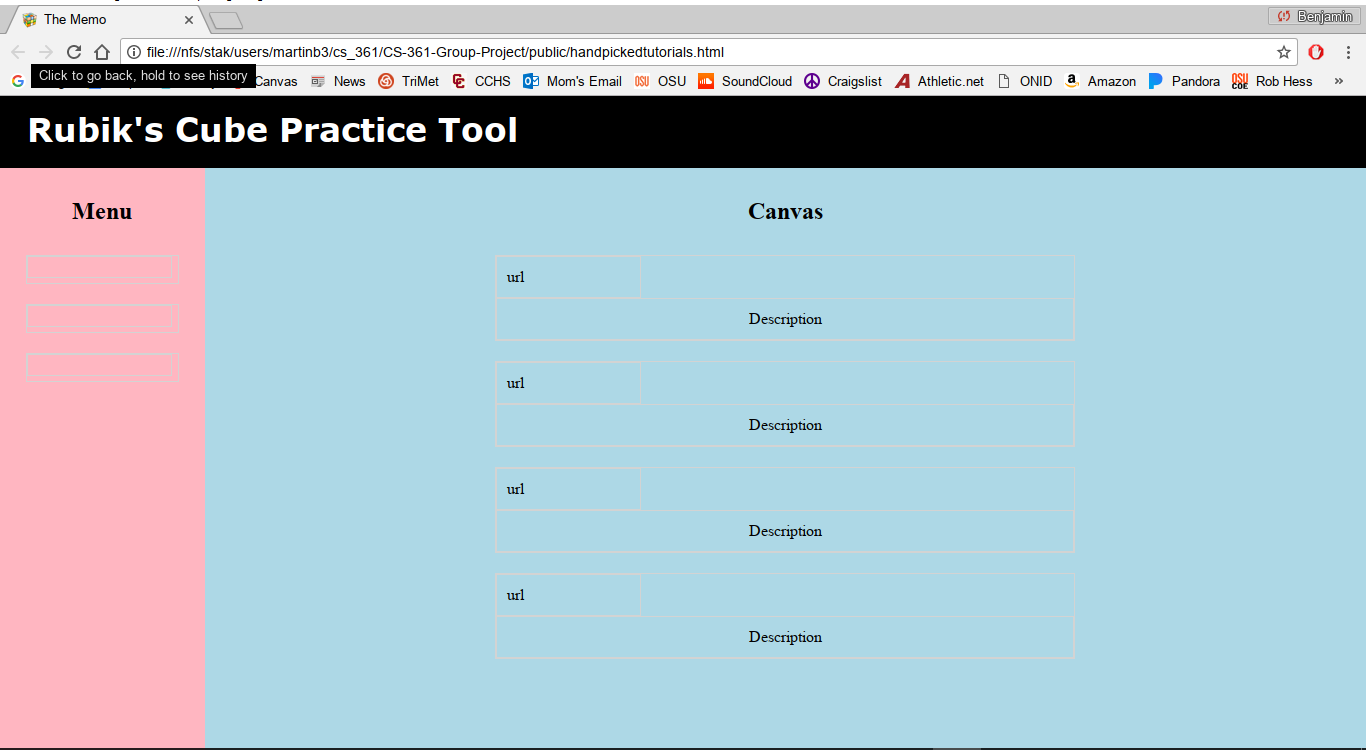
\includegraphics[width = \textwidth]{tutorial.PNG}
	\par
	On the canvas region of the tutorials page, there will be hotlinks to direct the user to tutorials to learn about how to solve the cube blindfolded. Since any new visitor that comes to this website may not be familiar with how to solve a Rubik's Cube blindfolded, this page is set as the HOME PAGE. This will be the first thing a user sees when they enter our website. If they are familiar with how to solve a Rubik's Cube blindfolded, they will proceed by clicking on a menu button on the left to navigate to other pages to practice their blindfolded skills. If they are not familiar, then they will click on the links to learn about how to solve a Rubik's Cube blindfolded. The choice is theirs to make on judging the sufficiency of their knowledge. \\
	
	\subsection{Rubik's Cube practice page}
	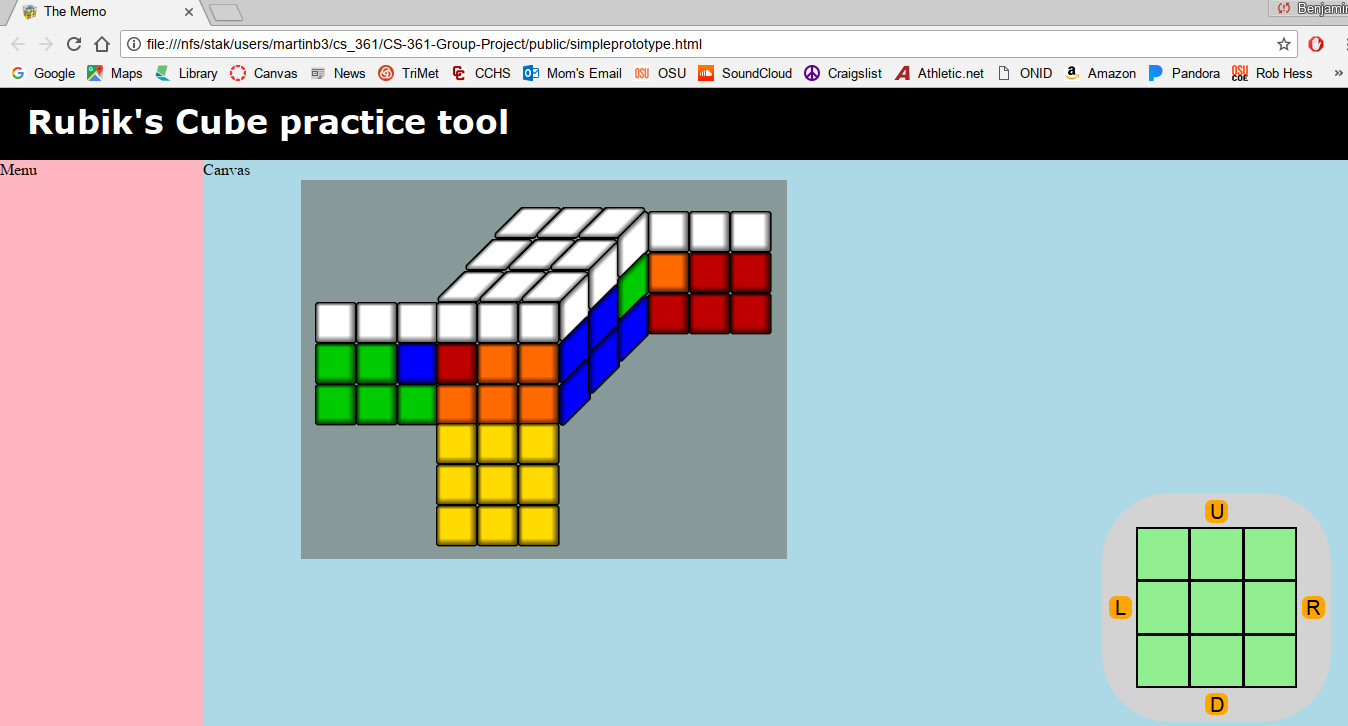
\includegraphics[width = \textwidth]{cubepage.PNG}
	\par
	This page will have a Rubik's Cube display (shaded in a dark grey background), and a "viewtoggle" display (the display in the bottom right hand corner). The viewtoggle will have four orthognal buttons to allow the user to rotate the face of the cube to see other sides. The Rubik's Cube display will also change accordingly to the button pressed on the viewtoggle. If, for example, the user were to press the "U" button, the cube display would rotate up, shifting all of the squares on each face down by one face. The squares colored on the viewtoggle would change as appropriate as well. The behavior of the changing colors of the cube would be determined by the cube object which will be described in detail in our diagrams. \\
	
	\subsection{Letter memorization page}
	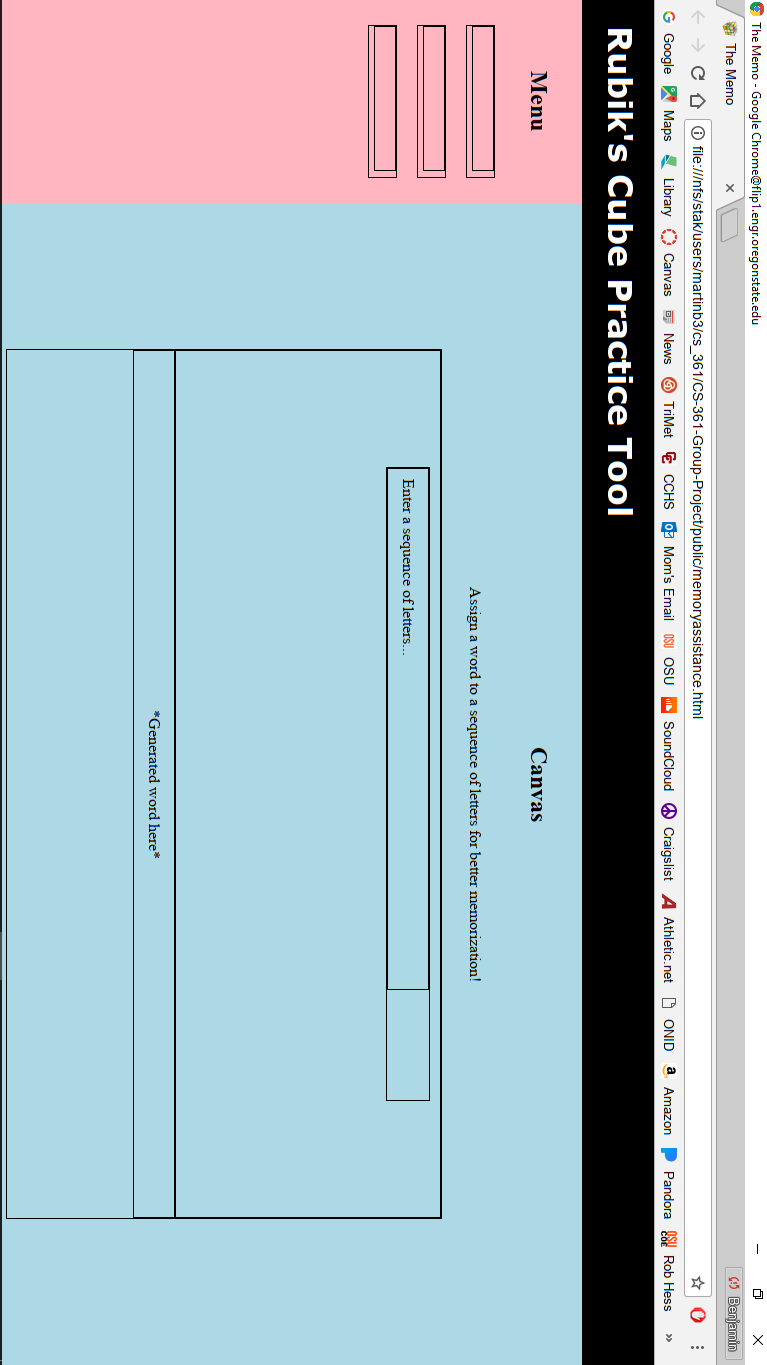
\includegraphics[width = \textwidth]{lettermem.PNG}
	\par
	The letter memorization page is simpler. There is a text box area where the user will input their string of letters. The user will then press the "Generate words" button, where the algorithm will then generate a random series of words from the letters given and display them on the canvas below the text input. The user can then repeat as many times as they feel like. If numbers or symbols are input there will be an alert from the webpage saying "Error" input is not valid!" and will NOT generate a string of words. \\

	
\includegraphics[width = \textwidth]{error.PNG}

\section{Class Diagrams}

	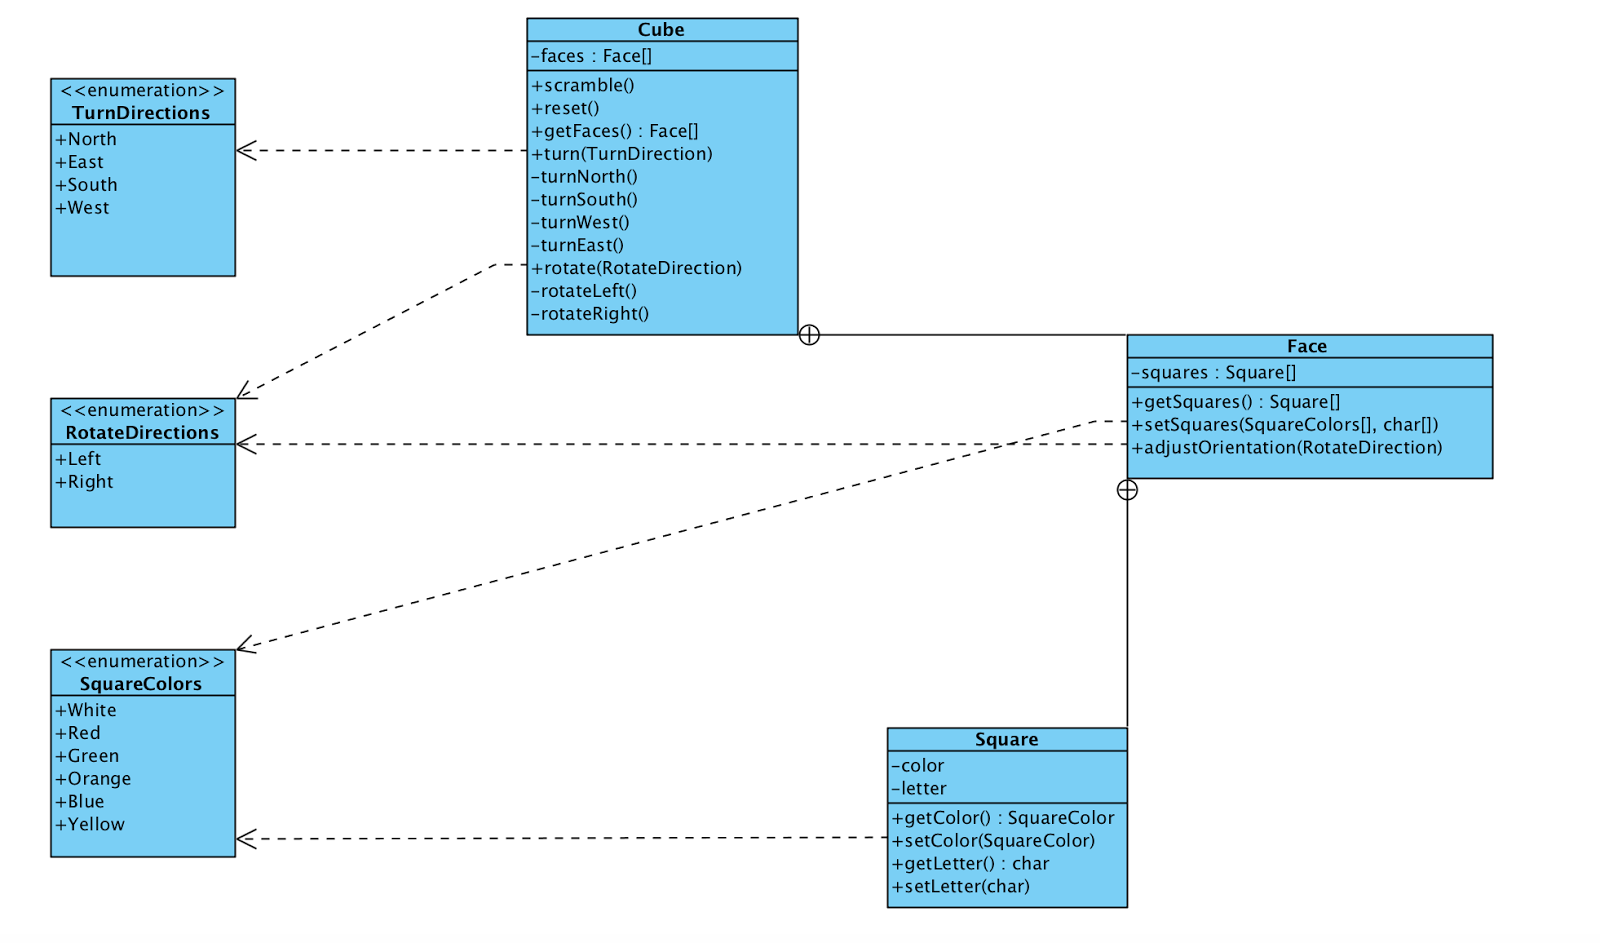
\includegraphics[width = \textwidth]{diagram.PNG}
	

\section{Sequence Diagrams}

	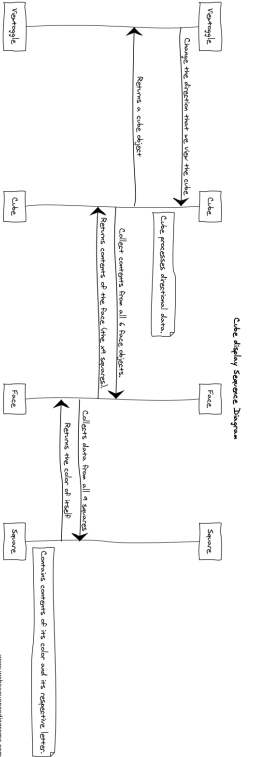
\includegraphics[width = \textwidth]{sequence.PNG}

\section{Meeting Report}

\par
On this week we have met 4 times on campus. Including three times in library and one meeting after class. \\

\par
On our first meeting on Wednesday. We met everyone in the library. we separate our second phase of the project to every group member. Jesse Chick is working on Class Diagrams. Benjamin Martin is working on Sequence Diagrams. Jiaji Sun is working on meeting report. Nickoli Londura is working on part of User Interface Prototypes. Keenan Johnson is working on scramble code and solution generation. On this meeting, we have drawn basic prototype of our project, and basic design each functions for every function. At the beginning, we drew a basic section of the prototype on paper, then rough design each functions for every function. Then we modify the design multiple times. Finally, we settle down the first version of the project. On this meeting, we find a new feature about our project is we implement one that generates easy to memorize words for given letter pairs. Example: given the letter pair CT would output an easy to memorize word such as ‘cat’. At the end of this meeting, we set up next meeting time. \\

\par
On our second meeting, we met after class. Everyone describes new idea of each other. We are thinking about the new design of our project, and everyone has talked about their new idea of our project. After we discussed our new design. We decide to keep discussed our project design at next meeting. Then we set next meeting time. \\

\par
On our third meeting, we met everyone in the library. we decide change design for our project. Jesse start modifies class diagrams into a new design. Benjamin also modifies his sequence diagrams into a new design. Nickoli starts working on the first version of prototypes of the project. Keenan is working on try to making code work well and smoothly. After we changed our design, the new version of our project design is come out. \\

\par
On our fourth meeting, we still met in the library. We have discussed our last version of project design and final version of prototypes. Jesse keeps working on class diagrams. Benjamin keeps working on sequence diagrams. Nickoli keeps working on the prototypes of our project. Keenan compiled every code to make sure it works well. At the end, Jesse and Benjamin finished their diagrams. Nickoli finished the prototypes of the project. Keenan compiled every code, and make every code working well. We have done our parts nicely. \\

\cite{rubtut}

\bibliography{myref}
\bibliographystyle{plain}

\end{document}
